% !TeX spellcheck = en_US

% We need layers to draw the block diagram
\usetikzlibrary{calc,positioning}
\usetikzlibrary{arrows.meta}

% Define a few styles and constants
\tikzstyle{entry}=[draw, minimum height=2em, align=center]
\tikzstyle{mytext}=[align=center]
\tikzstyle{frame} = [entry, text width=28em, fill=white,minimum height=10em, rounded corners]
\tikzstyle{engine} = [entry, text width=7em, fill=white,minimum height=4em, rounded corners, left color=green!15!white, right color=green!20!white,shading angle=135, anchor=north]
\tikzstyle{store} = [entry, text width=16em, fill=white,minimum height=6em, rounded corners, left color=blue!15!white, right color=blue!20!white,shading angle=135, anchor=north]
\tikzstyle{art} = [entry, text width=5em, fill=white,minimum height=3em, rounded corners, left color=red!15!white, right color=red!20!white,shading angle=135, anchor=north]
\def\blockdist{2.3}
\def\edgedist{2.5}

\begin{figure}
	\centering
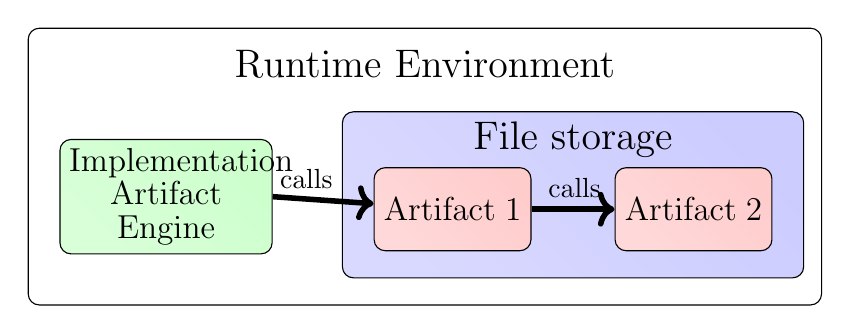
\begin{tikzpicture}
\node (frame) [frame, label={[shift={(+0ex,-5ex)}]north:{\Large Runtime Environment}}] {};

\node (engine) [xshift=+5em, yshift=+1em] at (frame.west) [engine] {\large Implementation Artifact Engine};
\node (storage) [xshift=-9em, yshift=+2em] at (frame.east) [store,label={[yshift=-2em]north:{\Large File storage}} ] {};

\node (art1) [xshift=+4em, yshift=+1em] at (storage.west) [art] {\large Artifact 1};
\node (art2) [xshift=-4em, yshift=+1em] at (storage.east) [art] {\large Artifact 2};

\draw [->,scale=5,line width=2pt] (engine.east) --node [text width=2.5cm,midway,above ] {~~~~~~calls} (art1);
\draw [->,scale=5,line width=2pt] (art1.east) --node [text width=2.5cm,midway,above] {~~~~~~~~calls} (art2);

\end{tikzpicture} 
\caption{Bad artifacts call sequence} 	\label{fig:artart}
\end{figure}